\title{Deadline Driven Behavior in Intelligent Virtual Environments}
\author{
        Djura Smits
}
\date{\today}

\documentclass[11pt]{book}
\usepackage[labelfont={bf}, margin=1cm]{caption}
\usepackage{titling}

\usepackage[colorinlistoftodos, bordercolor=white, backgroundcolor=cyan]{todonotes}
\usepackage{booktabs}
\usepackage{hyperref}

\graphicspath{{.}{../results}}

\begin{document}
\listoftodos
\maketitle
 \chapter*{\centering Abstract}
\addcontentsline{toc}{chapter}{Abstract}
%\abstract
\maketitle
\newpage
 \chapter*{\centering Acknowledgements}
\addcontentsline{toc}{chapter}{Abstract}
\maketitle
I would like to thank my supervisors Philip Kerbush from TNO, and Arnoud Visser from the UvA. Furthermore, I would like to thank Ernst Bovenkamp for providing the data and videos from Rotterdam airport.
\newpage
\tableofcontents
\newpage

\section{Introduction}
%\todo[inline]{Extend introduction}
Ever since the horrible tragedies on 9/11, there has been an increased interest in reinforcing security in public environments. The recent advances in technology have increased the feasibility of many different methods. An important approach in this area of interest is the automatic detection of suspicious behavior from camera images. The approaches in this area can vary, but one important aspect that they have in common, is the necessity of camera footage to be able to test the approaches. Since it can be extremely tedious to collect and annotate this data it would be very rewarding to be able to generate testing data on the fly. It is beyond the scope of our research to get into what suspicious behavior looks like, to we like to focus on the behavior of "non-suspicious" people. Assuming that so-called "normal" people greatly outnumber terrorists, these suspicious people could be added in later with ease. In other words, we would like to be able to quickly generate crowds of people doing normal, everyday behavior.\\
Simulation of pedestrians is a widely studied subject. Many models have been created for the various characteristics that arise when multiple agents move around in the same area. Many uses can be thought of for pedestrian simulation. An important purpose for this could be for example to easily create a large amount of "normal" pedestrians (as opposed to "suspicious" pedestrians).  Suspicious pedestrians whose behavior is scripted by hand can then be placed in the environment to easily create artificial testing data for suspicious behavior detection algorithms and such. Furthermore, the addition of simulated virtual pedestrians can add realism to otherwise mostly empty battlefield scenarios.

Another way to look at the behavior of groups of pedestrians is to explicitly specify how they behave when they enter a certain type of situation. In our approach, we would like to be able to specify behavior by drawing situations on an environment. For example, when a food stand is present in the area, we would like to be able to indicate that the agents that are placed in the neighborhood of that stand are able to do certain food-buying behavior.

An additional requirement is that we would like to indicate a certain \emph{deadline} for an agent which is the time at which its goal is not reachable any more. This approach results in roughly two types of behavior, \emph{hurried} and \emph{relaxed}. When the deadline approaches, less and less actions are likely to be done, since actions that take much time would result in not reaching the goal in time.\\
We validated our model by mimicking certain behaviors found on Rotterdam airport. We chose Rotterdam airport because time restrictions are very prevalent in a departure hall like the one on Rotterdam airport.


%In many fields using simulation, the environments are empty except for the absolutely necessary parts of the simulation. However, the environment would look much more realistic if actual civilians would walk around. That is why SIMOBS was developed. SIMOBS is a plugin for the VR-Forces simulation application that makes it easy to quickly generate residential areas inhabited by families, and factories where these civilians go to work. However, at the moment these virtual pedestrians only walk from their houses to their work and back at fixed points in time. The purpose of this thesis is to extend this SIMOBS plugin to create more realistic behavior.

\subsection{SIMOBS}
SIMOBS is a plugin for the military simulation toolkit VR-forces (\url{http://www.mak.com/products/vrforces.php} It is a tool for generating and executing battlefield scenarios. SIMOBS is a plugin developed to quickly generate inhabitants of an area by drawing residential areas and plants on the map in VR-forces. The behavior of these inhabitants is determined by \emph{Daily Motion Patterns}, which specify where certain types of inhabitants need to go at specified times. This is the idea that forms the basis for our research.


%\todo[inline]{Tweak research question.}
\subsubsection{Research Question}
The question we are going to base this research around is the following:
\begin{quote}
How can an intelligent virtual environment for simulated pedestrians be extended to deal with time-restricted destinations?
\end{quote}
Some of these terms may need some clarification:
\begin{itemize}
%\item \emph{Distributed}:\\
 %We are using a distributed environment to simulate our pedestrians. This means that various tasks such as path planning can be delegated to other services and are not of our concern. Therefore, we can afford to focus more on higher level behavior.
\item \emph{Intelligent Virtual Environment}:\\
IVE is a broad term, but in this particular case we mean that a large portion of the intelligence needed for the pedestrians to walk around is placed in the environment, instead of in the pedestrians walking in it. There are different ways to construct an IVE, which is something we have to look at as well.

\item \emph{Time-restricted destinations}:\\
We would like to create a framework that is able to deal with departure hall-like situations. That means that pedestrians will have a destination (e.g. a train, or an airplane, etc.) that will be available for a limited amount of time (until it departs). It can also be used to create simulations with a pattern that is more realistic when run for a long period of time (such as a whole day). Furthermore, in many situations, only the time is known when the person has to arrive at his destination. In those cases it is more intuitive to define the time of arrival, instead of determining at what time someone has to leave his starting point. In the rest of the article, we will refer to these time restrictions as \emph{deadlines}.
\end{itemize}

We are going to solve this question by trying to answer the following subquestions:
\begin{itemize}
\item \emph{To what extent can pedestrians be simulated realisticly?}\\
If it were feasible to model the complete human brain, we would probably get the most lifelike behavior. However, since this is not possible, we have to simplify the model somehow. Models can be made in varying levels of complexity. Most often, a higher complexity means slower performance. That is why we have to think about getting the right balance between realism and performance. We also have to decide how we define realism. Do we take the inner model into account, or do we purely compare the resulting behavior to real people in similar situations?

\item \emph{How do we let the pedestrians make decisions based on time left to reach the destination?}\\
In situations such as departure halls, people have a destination (e.g. airplane, train) that is only available for a limited amount of time. Some actions might take a very short amount of time, some may need more. How do we let these pedestrians decide between the different options?

%\item \emph{What kind of freedoms/restrictions do distributed systems give us?}\\
%As a consequence of using a distributed system we can delegate certain tasks to other units. On the other hand, our model also %needs to be compatible with the other units in the distributed system.

\item \emph{Is it possible to quickly generate these virtual pedestrians without much tweaking for each environment?}\\
We aim at creating pedestrians that can be used in many different environments without much additional scripting. Is it possible to do this and still have varied behavior between environments?
%\item How can the simulation be efficient without sacrificing too much realism?
\end{itemize}

%How do we create an \emph{intelligent virtual environment} framework so that \emph{realistic}, real-time acting virtual pedestrians can be generated \emph{quickly}, working with VR-forces and \emph{daily motion patterns}?
%\end{quote}
%Some terms will need some clarification about how we interpret them:
%\begin{itemize}
%\item \emph{Intelligent Virtual Environment}\\
%In an intelligent virtual environment, objects contain the rules about interacting with them, instead of the pedestrians.
%\item \emph{Realistic}:\\
%Crowds should move in a somewhat realistic manner and interact with the environment. Individuals should follow a logical path, making seemingly logical choices about what objects to interact with. Realistic refers to how the pedestrians act, not to their decision making model.
%\item \emph{Quick}:\\
%Requires as little specification as possible. Same specification for pedestrians have to be appropriate in many different environments.
%\item \emph{Daily Motion Patterns}:\\
%Things about the framework can be changed, but it may be preferrable to leave the Daily Motion Patterns in. DMPs require that pedestrians go to certain locations at certain times of the day.
%\end{itemize}

%This main question leads to a range of subquestions.
%\begin{quote}
%How do we balance realism and performance?
%\end{quote}
%How many pedestrians do we want to move around at the same time? How far does this limit the complexity of the models we can use?
%\begin{quote}
%How do we handle the planning?
%\end{quote}
%Daily motion patterns require the virtual pedestrians to be at a certain location at a certain time. How do we let the pedestrian decide for instance whether to go buy food or go to its train because it is almost leaving? Do we need to implement a model to handle basic needs such as hunger, and sleep, or will the pedestrians be able to act convincingly in another way?
%\begin{quote}
%What kinds of limits does the VR-forces framework give us?
%\end{quote}
%Our virtual pedestrians have to walk around in the VR-forces environment. This information has to be communicated to VR-forces in a certain way. This might restrict the possibilities of the simulation.


\section{Related Work}
% Tried to add tuples, but if I try to describe any more approaches with tuples, it would be like comparing apples and oranges.
%\todo[inline]{Indicate tuples for every approach (as much as is possible).}
When studying existing methods for modeling pedestrian behavior, the amount of available literature is quite overwhelming. This is not surprising as a large part of AI research focuses on the imitation of human behavior. However, not all means of simulating pedestrian behavior are developed for the same purpose. What we would like to have in our system, is a method to design behavior in an environment in the same way that other objects in the environment are designed. That is, it should be possible to spatially place the behaviors in the environment. However, this does not limit our search much since it only divides our desired result into two layers; namely the overall structure of different behaviors placed in the environment, and the definition of these different behaviors. When we approach the subject as \emph{designing behavior in an environment}, the search becomes much more narrow and directed.

\subsection{Designing the Situational Behaviors}
In our research, we can divide the subject of "behavior" in two layers.  First of all, we have the layer in which individual behaviors are described. However, this information is embedded in a framework that describes how these individual behaviors vary spatially. Let us start with focussing on these individual behaviors. This field knows many approaches. First of all, the focus can lie on the group as a whole. The different members of the group are then often viewed as particles that influence the other group members near them with attracting and repulsive forces. Other approaches view crowds as a group of individuals, and the members are given some kind of simplified psychological model. The motivation behind this simplified model is that this will lead to complex behavior when many of these simple units are put together in a large crowd. This effect is known as \emph{emergence}.\\

\subsection{Group Interaction}
The research of interaction in groups started with Reynolds' boids \cite{Reynolds87flocks} , where members of the group were seen as particles that exert both repulsive and attracting forces on the other members of the flock, depending on the distance to one another, and forces inwards from the outer contour of the flock, in order to remain in a certain shape.  This behavior is driven by three simple rules, namely \emph{separation} (avoiding crowding local flockmates), \emph{cohesion} (move toward center of mass of local flockmates), and \emph{alignment} (steering towards average heading of local flockmates). However, this flocking behavior is more suitable for modelling behavior of animals such as fish, and will not give a very plausible result when it is used to model humans. Because humans usually act in a way more complicated than a flock. However, many researches have built upon this idea of modelling large groups by viewing the members as particles.

\subsubsection{Global approaches}
Many models that have been proposed focus on crowds in panic situations. An example of a model for panic situations is the one proposed by Pelechano et al. \cite{citeulike1080090} who divided people in three categories: \emph{trained leaders}, who have complete knowledge about the building, \emph{untrained leaders}, who handle stress well, help others and will explore the building, and \emph{untrained non-leaders}, who might panic. \todo[inline]{Maybe sections have to be named differently, or previous reference has to be moved, the approach uses global effects, but also more individual models} Another example of simulating panic situations, can be found in the article of Helbing, Farkas, and Vicsek \cite{citeulike1656038}. In their model, people exert a repulsive interaction force to stay away from each other, an additional \emph{body force} slowing to counteract body compression, and a \emph{sliding friction force} when a pedestrian comes in contact with another pedestrian or the wall. This model can lead to several effects known to occur in real panic situations.\\
While these methods give a good insight into the movements in those particular panic situations, they are less suitable for experiments running over a longer period of time. Only in those few moments of panic, or when crowds are very dense, do these models represent a crowd realistically. What we are looking for, is a framework that gives realistic behavior over longer periods of time. Pelechano, Allbeck and Badler \cite{Pelechano:2007:CIA:1272690.1272705} have simulated high-density crowds for normal situations. They base the movement of the crowds on a simple wayfinding algorithm and a number of different psychological (impatience, panic, personality attributes, etc.) and physiological traits(e.g.locomotion and energy level). Furthermore, the agent is given perception and will react to objects and other pedestrians in the nearby space.\\
Bayazit, Lien and Amato approached the subject of crowd simulation in a very different way \cite{Bayazit02bettergroup}. Instead of letting an entity such as one pedestrian or a group do the navigation on the fly, global roadmaps are used. In this method, a map is generated beforehand defining where the pedestrians can walk. During simulation, the pedestrians are given a goal location, and will then explore the paths defined by the map, based on which direction exercises the highest force on the pedestrians. The pedestrians can update this map in real-time indicating if a path is favorable or not when trying to get to the goal. When two paths exert an equal amount of force on the pedestrians, they will split up and both paths will be explored simultaneously. This is the feature that makes this approach stand out from the rest. Because most of the previously mentioned techniques have less sophistication in the path planning of separate portions of the crowds. %\todo[inline]{This is not completely true, some panic approaches let the crowds explore, but probably had simpler navigation. Make the previous more nuanced}

However, global roadmaps are not the only way an environment can be divided. Various methods have been developed that use a combination of multi-agent techniques and cellular automata \cite{Dijkstra00amulti-agent}\cite{1241047}. Here, the behavior stems from a combination of basic multi-agent techniques, combined with information about how the pedestrians should be distributed over a grid. This grid follows the rules typical to cellular automata, where the value of a single square in the grid at time $t$ depends on the value of the surrounding grids at $t-1$.

%\todo[inline]{Maybe talk some more about cellular automata. But try to find a way that describes both articles.}

\subsubsection{Smaller Groups and Individual Approaches}
The previously mentioned approaches focus on movements of crowds as a whole. This might generate realistic effects when the crowds are very dense, but when the pedestrians are more sparsely scattered in the environment, these models will not suffice. That is why there have been many researches focusing more on crowds as a collection of smaller groups. In an urban environment, a lot of pedestrians move around together with a few other pedestrians and very few move around on their own. An important step in this direction has been made by Li, Jeng and Chang \cite{leaderfollower}, who proposed a leader-follower model, in which one person in a group gets the role of \emph{leader}, who has the job to decide on the destination and has to plan the path. This leader will exert an attractive force on the \emph{followers}, who will continuously follow this leader around. Hostetler and Kearny chose an approach in which all members of the group cast an equal vote on which direction to head in \cite{Hostetler02strollingdown}. The walkways have been modeled as ribbons to define the geometry of the surface, and wich create a conduit that channels pedestrian traffic into parallel streams. Every member of a group casts a vote on which way to turn and how to adjust the speed based on a discretized action space. The group will then collectively follow the action that has the highest vote. Peters, Ennis and O'Sullivan decided to have a more direct approach to the formation of groups \cite{10.1109MCG.2009.69}. They studied a large video corpus of prototypical walking areas and concluded groups always occur in certain formations. Subsequently, they designed a number of formations in a \emph{formation template} that represent discrete formations that the pedestrian groups may adopt, such as walking completely abreast, or in a staggered formation. The distance between the group members is defined by a cohesion matrix, which describes the cohesion between every two members in the group. Another factor contributing to the distance between each member is the minimum frontal aspect the formation can have, which describes the width of the formations.\\
Until now, we have only seen models that deal with crowds in terms of walking behavior. Interpersonal relationships may have been somewhat defined, but were only expressed through spacial positions. Bécheiraz and Thalmann have attempted to express these interpersonal dynamics through a set of animations that express a persons mood through body language \cite{Becheiraz:1996:MNC:791215.791499}.
%\todo[inline]{Clarify paper some more} Nah is pretty irrelevant I guess

\subsection{Interaction with Objects}
As previously mentioned, most researches with the focus on crowds as a group of individuals or viewed globally do not address the problem of how to interact with the environment except for some collision detection. This greatly reduces the realism of the simulation. The obvious solution is to extend the knowledge of the pedestrians with instructions about how to interact with these objects. This has been succesfully done for instance by Shao and Terzopoulos \cite{A_autonomouspedestrians}. They used an extensive psychological model to determine the behavior of the individuals. This led to a simulation in which the behavior looks very realistic, even when one invidual is followed for a long time. The downside to this method is that the behavioral model for the pedestrians has to be specifically crafted for the environment, which will be very time consuming. \\
It would be easier to generate the virtual human agents if the environment would automatically decide for the agents what interactions are possible and appropriate. The first step towards this focus was made by Kallmann and Thalmann who introduced the principle of \textit{smart objects} \cite{Kallmann98modelingobjects}.


\subsubsection{Mixed Approaches}
The distinction between larger and smaller groups is not black and white, as can be seen in the work of Braun et al. \cite{10.1109CASA.2003.1199317}, who generalized the model of Helbing, and introduced additional features for creating group behaviors, such as family members, dependence level, altruism level, and desired speed of the agent.\\
Farenc et al. even devised a hierarchical framework that incorporates a number of different models managing the crowd on different levels (crowd behavior, group specification, group behavior, and individual behavior). A framework such as this is very suitable for incorporating multiple crowd behavior techniques. While a single method of the previously mentioned techniques might not generate a satisfactory result, a hierarchic combination of several methods might be able to do the job.\\
Several other methods also have the potential to be extended to incorporate several other methods. For instance, it is very likely that the "situations" framework can be adapted to deal with higher level states, instead of the low-level animation-oriented states that are used now. It will then probably be possible to let situations incorporate certain effects (eg. a repulsive force) instead of simple animations. These effects could be one (or parts) of the previously mentioned other models.
\todo[inline]{Make sure the text fits better in the rest of the thesis}



\subsection{Designing the Behavior Structure in the Environment}
The approaches that fall under the previously mentioned categories generally focus on the general movement of crowds of pedestrians. However, when we want truly realistic behavior in a regular public environment, these methods do not suffice, because they miss interactions with objects in the environment. There are a few approaches that focus more on environment-dependent behavior, such as interaction with objects or situation-dependent actions.
The obvious solution is to extend the knowledge of the pedestrians with instructions about how to interact with these objects. This has been succesfully done for instance by Shao and Terzopoulos \cite{A_autonomouspedestrians}. They used an extensive psychological model to determine the behavior of the individuals. This led to a simulation in which the behavior looks very realistic, even when one invidual is followed for a long period of time. The downside to this method is that the behavioral model for the pedestrians have to be specifically crafted for the environment, which will be very time consuming.

We will now look at the behavior on the meta-level. A few methods have been developed to enable a user to design environment related behavior. The most obvious solution to specifying the behavior of pedestrians environment-dependently, is to craft a new script for the pedestrians for every new environment. However, this method is very inefficient when we make use of a larger set of environments. Therefore, we would like to be able to place the same pedestrians in different environments without creating a new script every time.  One method that deals with this problem uses so-called \emph{smart objects} in order to efficiently create behavior-rich environments. The main feature that makes the smart-objects method so efficient is that the information of how to interact with an object is completely contained within the object itself, and not in the agents. That is why the agents' behavior can easily be enriched by adding new smart objects in the environment.

In the most basic approach, these smart objects take complete control of the agents for a short period of time and let them interact with the object. The big advantage of this method is that the information for interacting with a specific object does not need to be stored in the pedestrians, but is stored in the objects themselves. This way, additional behavior can be added to a pedestrian by simply placing a new object in the environment.  The object also keeps track about how many agents can interact with it at the same time and if the interaction should be the same for all agents. For instance, an elevator modeled as a smart object will make the first agent interacting with it press the button, but not the next agents that approach this object. By using smart objects, the internal model of the pedestrians can be kept very simple, because they do not need to remember specific information about how to interact with the objects. Furthermore, this means that the pedestrians do not have to be specifically designed for the current simulation environment, because the environment will tell them how to act. In the most basic approach to smart objects, the agents lose all their autonomy when they approach a smart object. A lot of research has been built upon the idea of smart objects. For instance, Kallmann, de Sevin and Thalmann have extended this model to have agents that have their own motivations and needs \cite{Kallmann00constructingvirtual}. This model uses five main motivation types: eat, drink, rest, work, and go to toilet. These motivations control the action through a hierarchical decision graph. Information about which objects fulfill these different needs are added to the smart objects.\\






Another slightly different approach is the use of a situation based control structure (Sung, Gleicher and Chenny \cite{Sung04scalablebehaviors}). A situation is an area in the environment that requires the pedestrians to act in a certain way. The behavior of a pedestrian is described by a finite state machine in which a state is defined as follows:
 \[s = \{t, \bf{p}, \theta, s^- \}\]
In which $t$ is the time, $\bf{p}$ is the current position in two dimensional space, $\theta$ is the orientation, $a$ is an action, and $s^-$ is a list of previous states. By "action" they mean a particular animation clip that has to be played at this state. Situations extend the pedestrians' finite state machine with situation-specific actions. The probability distribution of the actions the pedestrian can take is multiplied with the probability distribution given by the situation. Situations are divided into two categories: \emph{spatial} situations for stationary objects or areas, and \emph{non-spatial} situations to describe concepts such as friendship with another pedestrian.



\subsection{General Behavior Modeling}
\subsubsection{Finite State Automata}
Finite-state machines (or finite state automata) are behavioral models that are composed of a number of states associated to transitions. A finite state machine moves from state to state by doing sets of actions associated with certain transitions. They are widely used in a variety of applications such as electronic design automation, but also for parsing.


\subsubsection{Petri Nets}
Petri nets are a mathematical modeling language used for the description of distributed systems. A petri net is a bipartite graph consisting of two types of nodes: places and transitions. These nodes are connected by directed arcs. An arc can run from either a place to a transition, or from a transistion node to a place, but never from a place to a place, or between two transitions. Activity in a Petri net is expressed by by the movement of tokens from place to place, through transitions. Input arcs (from place to transition) denote which places need to contain tokens in order to enable the transition. When a transition is enabled, it consumes the tokens from the input places, and produces tokens in the place indicated by the output arc.
Basic Petri nets can be described by a five-tuple:
\begin{equation}
PN = (P,T,I,O,M_0)
\end{equation}
which comprises of
\begin{itemize}
\item a set of places $P = (p_1, p_2, ..., p_m)$,
\item a set of transitions $T = (t_1, t_2, ...,o_m)$,
\item a set of input arcs $I \subset P \times T$,
\item a set of output arcs $O \subset T \times P$,
\item an initial marking $M_0 = (m_{01}. m_{02}, \ldots, m_{0m})$.

\end{itemize}

Petri nets have been extended in many ways in order to accomodate many different functionalities. The extention that attracts our attention the most is \emph{Stochastic Petri nets}. In this extension, there are two types of transitions: \emph{immediate} and \emph{timed} transitions.
The Stochastic Petri net (SPN) model can be described as a six-tuple:
\begin{equation}
SPN = (P,T,I,O,M_0,\Lambda)
\end{equation}
where $(P,T,I,O,M_0)$ is the marked untimed PN underlying the SPN, and $\Lambda = (\lambda_1, \lambda_2, \ldots, \lambda_n)$ is an array of (possibly marking dependent) firing rates associated with transitions.

Immediate transitions always have priority over timed transitions, and  the likelihood of firing a timed transition is dependent on a parameter called the \emph{firing rate} of the transition. This rate indicates the firing delay of the timed transition. This firing rate may be marking-dependent, so it should be written as $\lambda_i(M_j)$.  The average firing delay of a transition $t_i$ in marking $M_j$ is $[\lambda_i(M_j)]_{-1}$. Immediate transitions fire in zero time once they are enabled, while timed transitions fire after a random, exponentially distributed enabling time.

\subsubsection{Advantages of Petri Nets over Finite State Automata}
Petri nets hold several advantages over finite state automata. First of all, Petri nets allow for concurrent behavior. This would enable our pedestrians to do several tasks at once. For instance, it could be possible to model our pedestrians' Petri nets so that a token would represent an arm or a leg. That way, a pedestrian could execute multiple basic tasks independently. It would not be possible to achieve this kind of behavior with a finite state machine, unless a state would be described for every possible combination of activities.
However, this is not the only advantage Petri nets have over finite state automata. Petri nets come with a standardized way to incorporate a time aspect. For finite state automata, several techniques have been developed, but there is no general consensus over what methods are most suitable. The problem becomes even larger when we would like to incorporate both time and non-determinism. Both the aspects of time and non-determinism are easily incorporated in Petri nets with only small modifications, and can even be mixed with traditional Petri nets.
%A way to incorporate the decision of moving to the goal state or doing something else could be done by using tokens to represent time. These tokens should be used as a second input for every time-related transition. These tokens could be diminished for every unit of time, so certain transitions become inactive after a while because the time tokens that are needed for the input have run out.
An essential issue which has to be implemented in the method we are going to choose, is non-determinism. Fortunately, this is one of the basic properties of a Petri net. When multiple transitions are enabled at the same time, any of them may fire.\\
Lastly, availability will not be an issue either, since there are many packages for many languages freely available on the web.

\subsubsection{Are FSMs and Petri Nets interchangable?}
While finite state automata and Petri nets look very similar, there are some essential differences which make a direct mapping impossible. First of all, Petri nets enable us to work with concurrency. This means that usually, multiple transitions are enabled in one point in time. This could mean that the pedestrian should be able to do multiple activities at once. For example, a token could be created for certain parts of the pedestrian's body, such as for its hands and feet, or upper part and lower part.\\
Another issue that has to be dealt with is how the nets are going to be attached and detached from eachother. This could be done largely the same as with finite state automata, but Petri nets have the potential to do this in a much more versatile way. For example, situation petrinets could be designed to have different slots for pedestrians so that when multiple pedestrians use the situation at the same time, the pedestrians' Petri nets could be attached to the same situation Petri net at different places, which could be a convenient way to model several kinds of behavior involving multiple pedestrians such as queueing. An example of how this could be modeled can be found in figure \ref{restaurantnet}.
Customer 1 and customer 2 could be slots where a pedestrian's personal Petri net could be attached. \\
When we take an approach similar to this, there will be an important distinction between the Petri nets belonging to the pedestrians and situations. While there will be many identical pedestrian Petri nets in a simulation, there will be only one Petri net per instance of a situation. This might seem a trivial fact, but it is an important distinction between using finite state automata and Petri nets. When using finite state automata, every pedestrian will get a new instance of a situation's FSM attached to it. However, situation Petri nets will not multiply and will accept several pedestrians in their nets. This will make interaction between pedestrians in a situation a natural property of the system, in contrast to the FSM approach, where it will have to be implemented outside of the situations framework.

\begin{figure}
\begin{center}
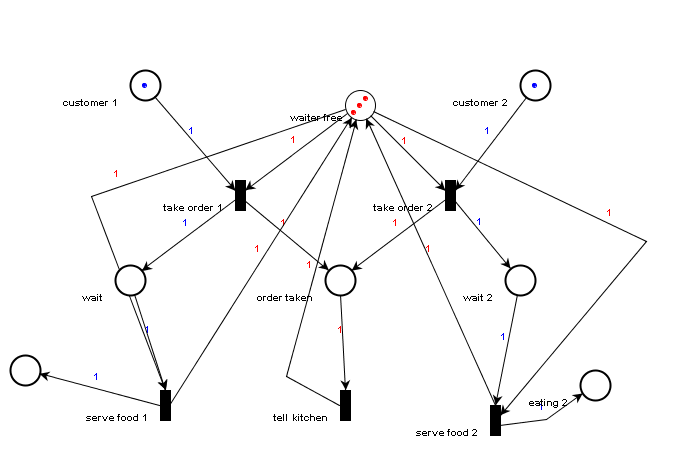
\includegraphics[width=450pt]{restaurant.png}
\label{restaurantnet}
\end{center}
\caption{An example of a behavioral model of a restaurant expressed in a Petri net}

\end{figure}

\subsection{Time Planning}
The essential extension to the situations framework that is proposed in this thesis adds an element of time to the system. This is needed to enable the system to deal with daily motion patterns. An important element without which the system cannot succeed is knowledge about how long actions are going to take. Only when this information is known to the agent (or system) it can be decided whether taking a certain action will result exceeding the deadline for the goal.


\subsection{Which Techniques Can We Use?}
We have seen many different techniques for many different purposes. We can immediately eliminate most global approaches to  crowds, since for most environments, we do not want the pedestrians to move as one big mass, all pedestrians heading into the same direction. Using purely attracting and repulsive forces will also generally not work when the pedestrians are too far apart, so we have another reason to rule out most global techniques. Of course, the global roadmaps approach does enable the pedestrians to split up and walk in different directions, but using this system on its own will not create very realistic behavior, since it does not have the capability to deal with interpersonal relations, and interaction with objects.
The techniques focusing on smaller groups do show some potential. Since most people move in smaller groups, this can lead to realistic effects. Ideally, people should interact with each other based on a variety of social relationships such as "parent" and "friend". However, this will require much configuration beforehand, and may increase processing time for each decision the pedestrians have to make. In this case, configuration may not be the issue, since these relationships can be defined and then used for many different simulations, but processing time is a larger problem, increasing with the number of pedestrians present in the simulation.
Of all the possible existing techniques, the "situations" approach of Sung et al. seems the most appealing. However, it is not directly usable for our purposes. One downside to the situations approach (at least how it is described in the paper) is that state transitions are mainly low-level animations. However, it should be possible to adapt the state transitions to correspond to higher-level actions, such as change of goal. Path planning should then be delegated to another module. In this way, it is very likely that the state representation can be reduced from $s = \{t, \bf{p}, \theta, s^- \}$ to $s = \{t, \bf{p}, \theta\}$. The $s^-$ was used to remember which actions were taken previously, so that the pedestrian remembers which way it was walking. When the actual walking is delegated to another module, it seems unnecessary to keep $s^-$.

\section{Method}
In the upcoming sections will be described how we decided to implement our system. We decided to base our model around the situations framework. We chose this framework because it allows for probabilistic behavior, and puts emphasis on defining behavior through the environment. This framework will have to be extended to deal with time restrictions. We will do this by replacing the finite state machines with Petri nets. However, we wont work with finite state machines, since these offer too little functionality to enable us to work with time restrictions. That is why we do the behavior modeling a little bit differently in our system. Instead of modeling the system with finite state machines, we describe the system with Petri nets.  The toolkit we will use for this is \emph{Platform Independent Petri net Editor 2} (PIPE2). \url{http://pipe2.sourceforge.net/} In the next section we describe how we decided to use this toolkit.

\subsection{PIPE2}
%\todo[inline]{Is this the place to discuss PIPE2 or should it be placed in the appendix?} Yes because having a toolkit to easily create those petri nets is pretty relevant.
PIPE2 is a tool written in Java to create and analyse petri nets. We chose this toolkit for a number of reasons. First of all, PIPE2 is written in Java, which makes it easier to integrate with our system. Secondly, this toolkit promised a number of Petri net extensions, the most important of which is the capability to create \emph{Generalized Stochastic Petri nets}. Generalized stochastic Petri nets is an extension that adds timed transitions to the modeling language.
%\todo{Name other reasons, since we don't use generalized stochastic petri nets any more}
Unfortunately, at a later time it seemed that the generalized stochastic petrinets did not behave as described in the specifications, so we decided to stick with modified, basic, untimed petri nets. Lastly, the PIPE2 toolkit has a clear, simple gui which can be used to create and modify Petri nets. This has been the main reason we chose this gui, because we wanted to create tools for easy modeling of behavior. It should be minimal effort to place large amounts of agents in a environment.
%\todo[inline]{Name disadvantages? Most disadvantages only become clear after PIPE2 has been used for a while so choosing PIPE was mostly because there was not enough time to extensively study alternatives, but it shouldn't be put like that.}


%This can be done by replacing the regular probabilistic finite state automata with probabilistic \emph{timed} state automata. Furthermore, we will be building an additional layer on the situations framework which will deal with with the \emph{needs} of the pedestrians. The list of needs a pedestrian will have will be dependent on which needs are defined in the situations in the environment. If, for instance, the environment contains a "food stand" situation, in which is specified that it defines the "hunger" need, pedestrians will act on this need. Whereas when the pedestrians are placed in an environment where for instance no food stands exist, and the "hunger" need cannot be fulfilled, pedestrians will not have this need at all.
 \todo[inline]{Extend introduction.}

\subsection{Pedestrian Layer}
Some drastic changes will be made in order to adapt the situations framework to our needs. Instead of using regular finite state automata, we use Petri nets so that environments in which time constraints are important (e.g. train stations, airports, etc. ) can be properly dealt with.

%\subsubsection{Probabilistic Timed State Automata}
%In the approach of Sung et al., regular probabilistic finite state automata are used. However, this is not sufficient when dealing with time-constrained goals. This is why we use a system called probabilistic timed automata. Probabilistic timed automata are an extension to B\"{u}chi automata which in turn are an extension to finite state automata. B\"{u}chi automata extend finite state automata to infinite inputs. Probabilistic timed automata use the acceptance conditions used in B\"{u}chi automata and extend these by using clocks, which can be incremented or reset. These clocks can be incorporated in the acceptance conditions, so that %transitions can be restricted based on time.

%\subsubsection{Time Planning}
%Our most important addition to the situations framework will be the aspect of time planning. This is going to be realised by %restricting the petrinets to follow a certain structure, so the time to the goal can be computed with the guarantee that a %path to the goal can be found relatively fast
%\todo[inline]{Elaborate on "fast"}
%Our approach is centered around the idea that the Petri nets designed for the standard pedestrian behavior all include a %"base" place. All regular tokens have to eventually return to this base place. Another important aspect of this place is that it %is directly connected to the transition that leads to the goal place. This way, searching for sequences of behaviors leading %to the goal place in time is greatly simplified.

%\todo[inline]{Refine following text}
%The general gist is that we use the idea of Beauquiers probabilistic timed automata \cite{Beauquier03}. Which means we %assign clocks to transitions and a transition is only accepted when the clock condition holds, and we use probabilistic %transitions, but we wont use the whole MDP problem solving part.

\subsubsection{Time Planning}
The fact that we use Petri nets with timed transitions, instead of finite state automata does not necessarily mean our pedestrians are able to deal with time constraints. However, these Petri nets have helped making our problem representable. In order to use these stochastic Petri nets efficiently for making decisions based on time constraints, we have made a number of assumptions.\\
First of all, we assume there are certain \emph{base places} from which it is always possible to reach the (time constrained) goal. Then, we will compute for every transition that will not take the pedestrian to its goal, how much time it takes to get back to the base state. Then we can check whether the goal place is still accessible from the base state when a certain transition has been taken. We use this information to modify the timed transition rate, so pedestrians are more likely to choose the actions that leave them more time to reach their goal.
As one may have noticed, this approach does not give a completely watertight solution to the planning problem. However, since we have to be able to model large crowds, we cannot create an overly complex planning system, since we would not be able to run the simulation real-time. Furthermore, we do not aim at finding an optimal solution to the planning problem, but rather the most lifelike behavior. In real life, people make errors in judgement, so creating pedestrians who can look ahead perfectly would not be realistic. It is impossible to make an exact definition of realism for our purposes, but what we try to do, is to copy certain specific behavior found in real-life footage. In our experiments we will try different functions for computing the probability of going to the goal, and attempt to assess which function will be most suitable.



\subsection{Assumptions}
The method we propose is based on various assumptions which have to be clarified. An important assumption is that the environment the pedestrians have to walk in are designed in such a way that it helps creating realistic behavior. This means that situations have to be defined in such a way that pedestrians will walk into them and act in the appropriate way. This makes our framework probably limited to certain kinds of environments. When an environment does not contain many situation areas or if they are too far apart, it is very likely that the framework does not give a satisfactory result.
Another assumption we make is that the pedestrians have to be at a certain place at a certain time. This makes the system more suitable for daily routine type situations rather than cases in which pedestrians are walking around without a proper goal. However, most situations can be described as having a deadline (e.g. eventually, most people have to go to bed), so this assumption is not necessarily very restrictive.\\
Furthermore, we assume that the behavior of the pedestrians can be described as finite state automata,  and that these automata incorporate base states to which transitions loop back, and from which it is always possible to reach the goal state (given enough time is left). We need this assumption in order to create an efficient way of determining which actions can be done before the deadline. Otherwise we would have to search through the finite state automaton in order to find the various ways actions can be tied together.\\

\subsection{Preparations}
Because the proposed system needs to run real-time, we refrain from overly complex systems that take too much computation power.
However, it is possible to do some computations before running the simulation, and save this for use during the simulation. An important application is the calculation of the distance in time between all the places in a Petri net and the goal place. This distance can easily be computed using the \emph{Dijkstra shortest path algorithm} \cite{dijkstra}. Dijkstra's algorithm is a graph search algorithm that can produce a shortest path tree for a single source, for a graph with nonnegative edges. In our system we can use this to compute the time from any place to the goal place (the source). This can be very useful when we would like to compute an estimate of how long a pedestrian will be stuck to the behavior of a certain situation. However, it will never be more than an estimate, since it is possible to design Petri nets with (possibly) infinite loops. But since the Petri nets are probabilistic, it will never be possible to give an exact prediction of the time it takes to execute a certain behavior.

The use of Dijkstra's algorithm does limit the use of our Petri nets though. For our simple implementation of Dijkstra's algorithm to be effective, we cannot use the Petri nets' more advanced features such as colored tokens.

\begin{itemize}
\item Write about problems with dijksta and petri nets, such as multiple tokens/slots, and colored tokens etc.
\end{itemize}



\section{Experiments}
Allthough it can be difficult to decide whether a group of people walks around "realistically", we will certainly give it a try. We will attempt to test our framework in two different ways; first of all, we will assess our framework by doing a qualitative comparison with real-life footage of Rotterdam Airport. We have access to both camera footage and manually annotated locations of the visitors. Secondly, we will assess how the the different probability functions we choose for the go-to-goal action will affect the frequency of other actions. In other words, we will attempt to investigat whether our method leads to \emph{emergent}  behavior.

\todo[inline]{Specify missing parameters}

\subsubsection{The Behaviors}

\paragraph{Going to the toilet}
In the videos, we observed that a typical behavior that manifests itself multiple times in the video material is that one person goes to the toilet, and another one waits until this person has come back. The Petri net used for this can be found in figure \ref{toiletsituation}.

\paragraph{Standing in the queue for the check-in desk}
\todo[inline]{This paragraph should probably be removed since we dont use it any more}
One constant factor in the video material seemed to be the people lining up in front of the check-in desk. There are many ways to model this behavior with our framework.
\todo{Mention other ways to model this}
We decided to split this behavior in two situations. First of all, we have the check-in situation, which in our simulation comes down to standing in front of the check-in desk for a short period of time. The other half of this behavior is the queue situation. This is an area in the hall where people line up with the people in front of them. The situation area is chosen such that the pedestrians in it will together form an orderly line. This means that the situation should not be too broad.


\paragraph{Checking in}
When the pedestrians reach the end of the queue situation, they will enter the check-in situation, in which they will stand in front of the check-in desk for a little while, after which they are free to go again.

\paragraph{Lean Against Pillar}
Another recurring behavior we saw is that people lean against the pillars in the hall. This is a type of idle behavior, a variation on the standing still behavior.

\paragraph{Wander}
One crucial behavior is missing. How are the pedestrians going to reach the different situation areas? This is only possible if they already have a move to begin with, otherwise they are only going to stay in place. That is why we added the \emph{wander} behavior. This behavior lets the pedestrian turn a random amount of degrees between $-45\pi$ and $45\pi$ and walk a few steps in that direction.

\subsection{Quantitative Experiment}
It is very difficult to quantitatively establish whether lifelike behavior has been modeled. However, it is possible to check whether the mechanics of time planning work as predicted. In order to do this, we log the pedestrian's relative time when they arrive at their goal to check how much time they had left until their deadline. If the model works correctly, this time should roughly correlate to how the time probability function has been chosen. We will discuss the various functions we have used to model the probabilities over time.

\subsubsection{Sigmoid Function}
A sigmoid function is an S-shaped curve that has a progression that accellerates and approaches a climax over time. This function can be found in many natural processes, such as learning curves. This function closely resembles how we reason that the behavior will shift when a pedestrian approaches a deadline.
A sigmoid function is defined as follows:
\begin{equation}
P(t) = \frac{1}{1+e^{-t}}
\end{equation}
% When the deadline is far away, it does not matter much whether the pedestrian goes straight to its goal or does something else. Even if time shifts a little, it still does not matter much. However, when the pedestrian moves on

%\begin{figure}
%\centering
%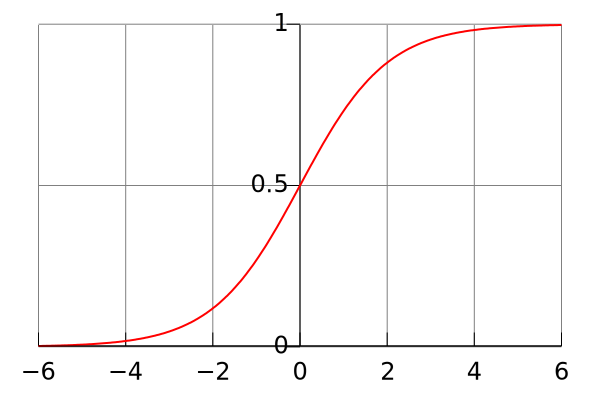
\includegraphics[width=200pt]{Logistic-curve}
%\caption{A typical sigmoid function}
%\label{sigmoid-example}
%\end{figure}

\subsubsection{Predictions for Behavior Using the Sigmoid Function}


\subsubsection{Linear Function}
We first chose to use a sigmoid function, because intuitively it felt like it would reflect real-life behavior best. However, it could be the case that the sophistication of this function is lost in practice. If this is the case, we might as well use the simpler linear function. We will use this function to check the necessity of the sigmoid function.

\subsubsection{Predictions for Behavior Using the Linear Function}

\subsubsection{Results for Linear Function}
It turns out a linear function gives significantly different behavior than a sigmoid function. Because there is a constant rise in the probability of walking to the goal, the pedestrians reach the goal very early, since there is a chance to go there every step, and this chance steadily increases. So all pedestrians have reached the goal long before the deadline. This is because the cumulative probability of the pedestrian going to the goal is very high very early.

\subsubsection{Gaussian Function}
We also used a Gaussian function to model the behavior. A Gaussian function is defined as follows:
\begin{equation}f(x) = ae^{- \frac{(x-b)^2}{2c^2}}\end{equation}
Where real constants $a, b, c > 0 $. A Gaussian distribution (or normal distribution) is a continuous probability distribution with a bell-shaped probability density function which have a mean and variance as parameters.


\subsubsection{Predictions for Behavior Using the Gaussian Function}
We chose to try a Gaussian function as well because of the following reasoning: A pedestrian might not care about going to it's goal until it is approximately the time of the deadline. With this we mean that going to the goal is a priority \emph{around} the time of the deadline, and will also decline when the deadline has passed for a while, and the pedestrian hasn't reached its goal yet. With this reasoning, the "go-to-goal" behavior frequency should increase when approaching the deadline, and should peak \emph{just} before the deadline, and declines thereafter.

\subsubsection{Results for Gaussian Function}


\subsubsection{What can we derive from these results?}
From these results, we can see that not only does the changing of the goal probability function affect the time at which the agents decide when to move to the goal, but also the time at which other actions are executed. This shows that our framework is able to generate emergent behavior. When the probability of going to the goal is high, actions that take longer to finish have a very low frequency.

\subsection{Qualitative Experiment}
Apart from quantitative analysis, we will also qualitatively judge the pedestrians' behavior. We will do this by comparing our modeled behavior with real-life behavior from recordings of Rotterdam airport. We have picked a couple of specific behaviors that we have modeled with our system.

\subsubsection{The Dataset}
We acquired manually annotated data indicating the tracks of the visitors of Rotterdam airport. 


\subsection{Results}
Below you will find the results of the quantitative experiment, where we used a variety of functions to check whether emergent behavior occurs.

In figure \ref{evaluation_log_linear0point2automatedpointcsv}, you can see the results of choosing a linear function from 0 to 0.2 as the goal probability function. We can see here that the pedestrians reach their goal very early, that is, 100 \% of the pedestrians reach the goal so early, they could easily have used the remaining time to do a multitude of other activities.

\todo[inline]{Aggegrate graphs}
\begin{figure}
\centering
\includegraphics[width=250pt]{./automaticResults/evaluation_log_linear0point2automatedpointcsv.png}
\caption{evaluation\_log\_linear0point2automatedpointcsv}
\label{evaluation_log_linear0point2automatedpointcsv}
\end{figure}

In figure \ref{evaluation_log_linear0point5automatedpointcsv} the same effect can be seen even more exaggerated. Again, we see that the linear probability function causes the pedestrians to arrive at their goal way too early.

\begin{figure}
\centering
\includegraphics[width=250pt]{./automaticResults/evaluation_log_linear0point5automatedpointcsv.png}
\caption{evaluation\_log\_linear0point5automatedpointcsv}
\label{evaluation_log_linear0point5automatedpointcsv}
\end{figure}

\begin{figure}
\centering
\includegraphics[width=250pt]{./automaticResults/evaluation_log_linear1automatedpointcsv.png}
%\caption{The global workings of our framework}
\label{evaluation_log_linear1automatedpointcsv}
\end{figure}

In figure \ref{evaluation_log_sigmoid0point01automatedpointcsv} we see the results of using a sigmoid for goal probability function with a minimum \todo[inline]{find out how to describe, since those values only count in the limit or whatever} of 0 and a maximum of 0.01. Again we see that a maximum probability of 0.01 is low to have the pedestrians reach their goal in time.

\begin{figure}
\centering
\includegraphics[width=250pt]{./automaticResults/evaluation_log_sigmoid0point01automatedpointcsv.png}
\caption{evaluation\_log\_sigmoid0point01automatedpointcsv}
\label{evaluation_log_sigmoid0point01automatedpointcsv}
\end{figure}



\begin{figure}
\centering
\includegraphics[width=250pt]{./automaticResults/evaluation_log_sigmoid0point1automatedpointcsv.png}
%\caption{The global workings of our framework}
caption{evaluation\_log\_sigmoid0point1automatedpointcsv}
\label{evaluation_log_sigmoid0point1automatedpointcsv}
\end{figure}

\begin{figure}
\centering
\includegraphics[width=250pt]{./automaticResults/evaluation_log_sigmoid0point2automatedpointcsv.png}
%\caption{The global workings of our framework}
\caption{evaluation\_log\_sigmoid0point2automatedpointcsv}
\label{evaluation_log_sigmoid0point2automatedpointcsv}
\end{figure}

\begin{figure}
\centering
\includegraphics[width=250pt]{./automaticResults/evaluation_log_sigmoid0point5automatedpointcsv.png}
%\caption{The global workings of our framework}
\caption{evaluation\_log\_sigmoid0point5automatedpointcsv}
\label{evaluation_log_sigmoid0point5automatedpointcsv}
\end{figure}

We can only say more about the results if the frequencies are divided by the total number of pedestrians in the simulation at that moment. The curve we see in figure \ref{evaluation_log_sigmoid0point01automatedpointcsv}, \ref{evaluation_log_sigmoid0point1automatedpointcsv}, \ref{evaluation_log_sigmoid0point2automatedpointcsv}, and \ref{evaluation_log_sigmoid0point5automatedpointcsv} (though to a lesser extent) can be explained by a multitude of causes. First of all, it can be explained by the fact that the number of pedestrians in the simulation diminishes as they finish their goal action. It could also be caused by the probability function increasing, but in this case, that is highly unlikely, because that would result in data quite opposite to the results here. Lastly, it could be that at certain moments, there are more pedestrians already engaged in other multi-step activities.


\subsection{Results 2}
Below follow the results of the other actions, that is, the actions that are not directly connected to the goal probability. The results of these actions have to show that our framework is also capable of generating \emph{emergent} behavior.

\begin{figure}
\centering
\includegraphics[width=250pt]{./automaticResults2/evaluation_log2_gaussian0point01twoPeopleToiletSituationpointxmlpointcsv.png}
%\caption{The global workings of our framework}
\label{evaluation_log2_gaussian0point01twoPeopleToiletSituationpointxmlpointcsv}
\end{figure}

\begin{figure}
\centering
\includegraphics[width=250pt]{./automaticResults2/evaluation_log2_gaussian0point2pillarSituationpointxmlpointcsv.png}
%\caption{The global workings of our framework}
\label{evaluation_log2_gaussian0point2pillarSituationpointxmlpointcsv}
\end{figure}

\begin{figure}
\centering
\includegraphics[width=250pt]{./automaticResults2/evaluation_log2_gaussian0point2standStillSituationpointxmlpointcsv.png}
%\caption{The global workings of our framework}
\label{evaluation_log2_gaussian0point2standStillSituationpointxmlpointcsv}
\end{figure}

\begin{figure}
\centering
\includegraphics[width=250pt]{./automaticResults2/evaluation_log2_gaussian0point2twoPeopleToiletSituationpointxmlpointcsv.png}
%\caption{The global workings of our framework}
\label{evaluation_log2_gaussian0point2twoPeopleToiletSituationpointxmlpointcsv}
\end{figure}

\begin{figure}
\centering
\includegraphics[width=250pt]{./automaticResults2/evaluation_log2_gaussian0point5pillarSituationpointxmlpointcsv.png}
%\caption{The global workings of our framework}
\label{evaluation_log2_gaussian0point5pillarSituationpointxmlpointcsv}
\end{figure}

\begin{figure}
\centering
\includegraphics[width=250pt]{./automaticResults2/evaluation_log2_gaussian0point5standStillSituationpointxmlpointcsv.png}
%\caption{The global workings of our framework}
\label{evaluation_log2_gaussian0point5standStillSituationpointxmlpointcsv}
\end{figure}

\begin{figure}
\centering
\includegraphics[width=250pt]{./automaticResults2/evaluation_log2_gaussian0point5twoPeopleToiletSituationpointxmlpointcsv.png}
%\caption{The global workings of our framework}
\label{evaluation_log2_gaussian0point5twoPeopleToiletSituationpointxmlpointcsv}
\end{figure}

\begin{figure}
\centering
\includegraphics[width=250pt]{./automaticResults2/evaluation_log2_linear0point01automated-pillarSituationpointcsv.png}
%\caption{The global workings of our framework}
\label{evaluation_log2_linear0point01automated-pillarSituationpointcsv}
\end{figure}
\clearpage

\begin{figure}
\centering
\includegraphics[width=250pt]{./automaticResults2/evaluation_log2_linear0point01automated-standStillSituationpointcsv.png}
%\caption{The global workings of our framework}
\label{evaluation_log2_linear0point01automated-standStillSituationpointcsv}
\end{figure}

\begin{figure}
\centering
\includegraphics[width=250pt]{./automaticResults2/evaluation_log2_linear0point01automated-twoPeopleToiletSituationpointcsv.png}
%\caption{The global workings of our framework}
\label{evaluation_log2_linear0point01automated-twoPeopleToiletSituationpointcsv}
\end{figure}

\begin{figure}
\centering
\includegraphics[width=250pt]{./automaticResults2/evaluation_log2_linear0point1automated-standStillSituationpointcsv.png}
%\caption{The global workings of our framework}
\label{evaluation_log2_linear0point1automated-standStillSituationpointcsv}
\end{figure}

\begin{figure}
\centering
\includegraphics[width=250pt]{./automaticResults2/evaluation_log2_linear0point1automated-twoPeopleToiletSituationpointcsv.png}
%\caption{The global workings of our framework}
\label{evaluation_log2_linear0point1automated-twoPeopleToiletSituationpointcsv}
\end{figure}

\begin{figure}
\centering
\includegraphics[width=250pt]{./automaticResults2/evaluation_log2_linear0point2automatedstandStillSituationpointxmlpointcsv.png}
%\caption{The global workings of our framework}
\label{evaluation_log2_linear0point2automatedstandStillSituationpointxmlpointcsv}
\end{figure}

\begin{figure}
\centering
\includegraphics[width=250pt]{./automaticResults2/evaluation_log2_linear0point2automatedtwoPeopleToiletSituationpointxmlpointcsv.png}
%\caption{The global workings of our framework}
\label{evaluation_log2_linear0point2automatedtwoPeopleToiletSituationpointxmlpointcsv}
\end{figure}
\clearpage

\begin{figure}
\centering
\includegraphics[width=250pt]{./automaticResults2/evaluation_log2_linear0point5automatedtwoPeopleToiletSituationpointxmlpointcsv.png}
%\caption{The global workings of our framework}
\label{evaluation_log2_linear0point5automatedtwoPeopleToiletSituationpointxmlpointcsv}
\end{figure}

\begin{figure}
\centering
\includegraphics[width=250pt]{./automaticResults2/evaluation_log2_linear1automatedtwoPeopleToiletSituationpointxmlpointcsv.png}
%\caption{The global workings of our framework}
\label{evaluation_log2_linear1automatedtwoPeopleToiletSituationpointxmlpointcsv}
\end{figure}

\begin{figure}
\centering
\includegraphics[width=250pt]{./automaticResults2/evaluation_log2_sigmoid0point01automatedpillarSituationpointxmlpointcsv.png}
%\caption{The global workings of our framework}
\label{evaluation_log2_sigmoid0point01automatedpillarSituationpointxmlpointcsv}
\end{figure}

\begin{figure}
\centering
\includegraphics[width=250pt]{./automaticResults2/evaluation_log2_sigmoid0point01automatedstandStillSituationpointxmlpointcsv.png}
%\caption{The global workings of our framework}
\label{evaluation_log2_sigmoid0point01automatedstandStillSituationpointxmlpointcsv}
\end{figure}

\begin{figure}
\centering
\includegraphics[width=250pt]{./automaticResults2/evaluation_log2_sigmoid0point01automatedtwoPeopleToiletSituationpointxmlpointcsv.png}
%\caption{The global workings of our framework}
\label{evaluation_log2_sigmoid0point01automatedtwoPeopleToiletSituationpointxmlpointcsv}
\end{figure}

\begin{figure}
\centering
\includegraphics[width=250pt]{./automaticResults2/evaluation_log2sigmoid0point1automatedpillarSituationpointxmlpointcsv.png}
%\caption{The global workings of our framework}
\label{evaluation_log2sigmoid0point1automatedpillarSituationpointxmlpointcsv}
\end{figure}

\begin{figure}
\centering
\includegraphics[width=250pt]{./automaticResults2/evaluation_log2sigmoid0point1automatedstandStillSituationpointxmlpointcsv.png}
%\caption{The global workings of our framework}
\label{evaluation_log2sigmoid0point1automatedstandStillSituationpointxmlpointcsv}
\end{figure}
\clearpage

\begin{figure}
\centering
\includegraphics[width=250pt]{./automaticResults2/evaluation_log2sigmoid0point1automatedtwoPeopleToiletSituationpointxmlpointcsv.png}
%\caption{The global workings of our framework}
\label{evaluation_log2sigmoid0point1automatedtwoPeopleToiletSituationpointxmlpointcsv}
\end{figure}

\begin{figure}
\centering
\includegraphics[width=250pt]{./automaticResults2/evaluation_log2sigmoid0point5automatedpillarSituationpointxmlpointcsv.png}
%\caption{The global workings of our framework}
\label{evaluation_log2sigmoid0point5automatedpillarSituationpointxmlpointcsv}
\end{figure}

\begin{figure}
\centering
\includegraphics[width=250pt]{./automaticResults2/evaluation_log2sigmoid0point5automatedstandStillSituationpointxmlpointcsv.png}
%\caption{The global workings of our framework}
\label{evaluation_log2sigmoid0point5automatedstandStillSituationpointxmlpointcsv}
\end{figure}
\clearpage

\begin{figure}
\centering
\includegraphics[width=250pt]{./automaticResults2/evaluation_log2sigmoid0point5automatedtwoPeopleToiletSituationpointxmlpointcsv.png}
%\caption{The global workings of our framework}
\label{evaluation_log2sigmoid0point5automatedtwoPeopleToiletSituationpointxmlpointcsv}
\end{figure}

\begin{figure}
\centering
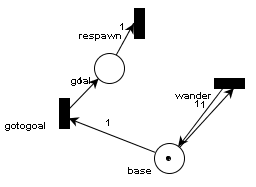
\includegraphics[width=200pt]{rotterdamPedestrianNet}
\caption{The basic petrinet for the pedestrian model for Rotterdam airport}
\label{basicnet}
\end{figure}

\begin{figure}
\centering
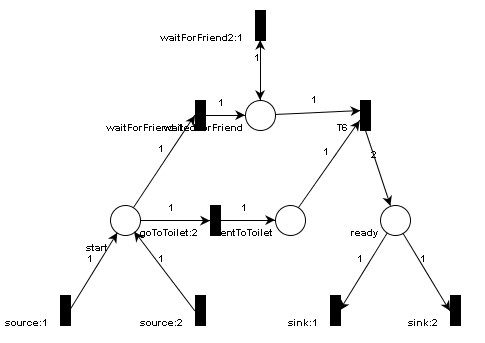
\includegraphics[width=350pt]{twoPeopleToiletSituation}
\caption{Behavior model for the toilet situation}
\label{toiletsituation}
\end{figure}

\begin{figure}
\centering
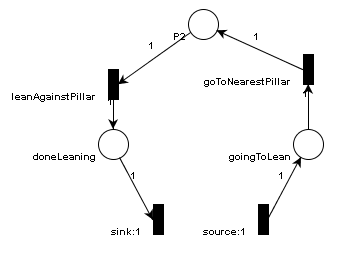
\includegraphics[width=250pt]{pillarSituation}
\caption{Behavior model for the pillar situation}
\label{toiletsituation}
\end{figure}


%\todo[inline]{The following is only a rough draft}
%It is very difficult to determine whether one has been successful at modeling lifelike behavior. What we are going to do is %study footage of real-life behavior at Rotterdam Airport, and pick out various behavioral patterns. Then, we are going to %model these patterns with our system.

\section{Conclusion \& Discussion}
The results are different from what we expected, but logical nonetheless. We expected the sigmoid function to have the ideal curve to reflect the behavior of the pedestrians in Rotterdam airport but


\subsection{Limits of the Deadline Driven Behavior Framework}
Modeling pedestrian behavior with our method does have its limits. First of all, the movements of the agents are designed explicitly through linking together basic movements in the Petri nets. As a consequence, interaction with other agents is quite static, and not directly responsive to surrounding agents. Consequently, our method is not particularly suitable for situations in which the pedestrians have to move very close together, such as when a large amount of pedestrians has to move through a narrow space and have to move closer together or form a queue. When pedestrians move very close together, their behavior will become more uniform, and it would be more sensible to look at the group as a whole, and not as individuals. A more suitable approach would then for example be to look at crowds as particles in a liquid, like Moore, Ali, Mehran and Shah have done \cite{Moore:2011:VCS:2043174.2043192}. Their supposition is that people in crowds seem to move according to the flow, just like particles in a liquid.

\subsection{Other things}
\todo[inline]{find better subtitle}
It is very well possible that the results found in our research are far from the optimal results we could have gotten with our framework.  Machine learning could be used to attain the optimal deadline driven behavior. However, this is beyond the scope of our research.


\subsection{Future Work}
There are several ways in which the deadline driven behavior framework can be extended. For example, currently, the probabilities for entering situations are only dependent on how close the agent is to the deadline. So, no matter what time of day it is, the pedestrians will always have the same probability to do a certain action. However, in real life, a person's probabilities for certain behavior is also largely dependent on their daily cycle.

\subsubsection{Needs}
Ideally, a pedestrian's propensity to execute certain actions, such as eating, should vary dependent on whether the individual has recently executed that action, and their daily cycle. In other words, we would like to introduce \emph{needs} to the framework. By introducing the concept of needs, we would be better able to model the daily flow of people in a typical public area. We can vary the needs according to the time of day and whether this need has been fulfilled recently.

\appendix

\section{Appendix A: Implementation}
In the appendix we will go into some of the details of implementation of the deadline driven behavior framework. We will also give some directions about how to use our implementation to simulate your own scenario, or to extend it yourself.


\subsection{Implementing the Framework}


\subsection{Extending PIPE2}

\subsubsection{Sources, Sinks, Slots}
In order to facilitate transporting tokens between Petri nets, we created classes of transitions with added functionality to keep track of how these nets are connected. These transitions are called \emph{sinks} and \emph{sources}. A source is a transition that has no incoming connections, only outgoing, with the result that this kind of transition produces new tokens without consuming any, increasing the total amount of tokens in the Petri net. A sink is exactly the opposite: it only consumes tokens and does not produce, effectively decreasing the amount of tokens in the network. Subsequently, we can use these special classes of transitions to transport tokens from one net to another. In order to keep track of how the nets are connected, we pair a sink with every source transition. These pairs are put together in a class called \emph{Slot}.

\subsubsection{Additional Modifications}


\subsection{MASON}

\subsection{Connecting MASON and the Situations Framework}
We deliberately divided our framework into two main modules. Because the situations framework has been implemented with the prospect of interfacing it with other simulations we decided to have the two main units communicate through socket connections. We have the situations side keep track of a thread pool. Every time a pedestrian from the MASON side connects to the situations side, a check is done whether this MASON pedestrian has connected to the Situations before. If this is not the case, another thread will be created to handle the connection to this new pedestrian.  Figure \ref{framework}  shows the global structure. Here you can see how the two interact.
\todo[inline]{Finish this part about MASON}
\begin{itemize}
\item Blabla thread pool
\item blabla 1 kant is niet multithreaded maar whatever
\item ...
\end{itemize}


\section{Appendix B: Results}
\begin{figure}
\centering
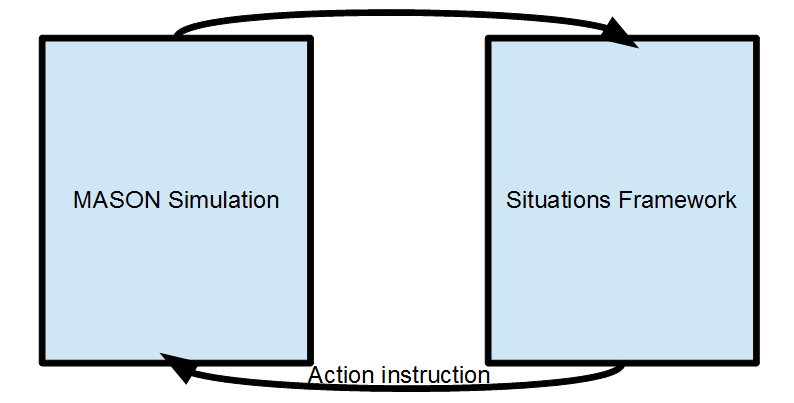
\includegraphics[width=250pt]{framework}
\caption{The global workings of our framework}
\label{framework}
\end{figure}



\bibliographystyle{plain}
\bibliography{references}

\todo[inline]{Check all references (figures, papers, etc.)}

\end{document}
